\documentclass[UTF8,ctexart,a4paper,11pt,openany]{article}
\usepackage[slantfont,boldfont]{xeCJK}
\usepackage{fontspec}
\usepackage{ctex}

\setCJKmainfont{SimSun}%[BoldFont=SimHei] %去掉注释:bf字体为黑体

\setsansfont{SimHei}
\setCJKsansfont{SimHei}

\xeCJKsetcharclass{"2160}{"2470}{1}% 1: CJK
\xeCJKsetup{AutoFallBack=true}
\setCJKfallbackfamilyfont{\CJKrmdefault}{SimSun.ttf}

%\setmainfont{Times New Roman}     %去掉注释:Times new roman字体
%\usepackage{mathptmx}             %去掉注释:Times new roman字体

\usepackage{mathtools}
\usepackage{amsmath}
\usepackage{amsfonts}
\usepackage{amssymb}
\usepackage{amsthm}
\usepackage[T1]{fontenc}
\usepackage{indentfirst} %段首空两格

\usepackage{graphicx}
\usepackage{geometry}
\usepackage{latexsym}
\usepackage{fancyhdr}
\usepackage{epstopdf}
%\usepackage{pifont}
%\usepackage[perpage,symbol*]{footmisc}
\usepackage{titlesec}
\usepackage{setspace}
\usepackage{enumerate}
\usepackage{enumitem}
\usepackage{multicol}
\usepackage{url}
\usepackage{exscale}
\usepackage{ulem}
\usepackage{relsize}
\usepackage{mathrsfs}
\usepackage{tikz}
\usepackage{wrapfig}
\usepackage{framed}
\usepackage{bm}
%\usepackage{pstricks,pst-node,multido,ifthen,calc}
\usepackage[all]{xy}
\usepackage{extarrows}
%\usepackage[backref]{hyperref}
\usepackage{hyperref}
\usepackage{stfloats} %插图的时候不分页

\setlength{\parindent}{2em} %段首空两格
\linespread{1.2}
\usepackage{listings}
\usepackage{xcolor}
\usepackage{algorithm}
\usepackage{algorithmicx}
\usepackage{algpseudocode}
\usepackage{mdframed}
\usepackage{extarrows}
\usepackage{diagbox}
\usepackage{makecell}

\theoremstyle{definition}
\mdfdefinestyle{theoremstyle}{%
linecolor=green!40,linewidth=.5pt,%
backgroundcolor=green!10,
skipabove=8pt,
skipbelow=5pt,
innerleftmargin=7pt,
innerrightmargin=7pt,
frametitlerule=true,%
frametitlerulewidth=.5pt,
frametitlebackgroundcolor=green!35,
frametitleaboveskip=0pt,
frametitlebelowskip=0pt,
innertopmargin=.4\baselineskip,
innerbottommargin=.4\baselineskip,
shadow=true,shadowsize=3pt,shadowcolor=black!20,
%theoremseparator={\hspace{1pt}},
theoremseparator={.},
nobreak=true,
}

\everymath{\displaystyle}

\newtheorem{definition}{\hspace{2em}定义}[section]
\newtheorem{axiom}{\hspace{2em}公理}
\newtheorem{lemma}[theorem]{\hspace{2em}引理}
\newtheorem{corollary}[theorem]{\hspace{2em}推论}

\mdtheorem[style=theoremstyle]{theorem}{定理}
\mdtheorem[style=theoremstyle]{example}{例}
\mdtheorem[style=theoremstyle]{exercise}{问题}

\newcommand*{\QED}{\hfill\ensuremath{\square}}
\newcommand*{\rmk}{\textbf{注:}}
\renewcommand*{\proof}{\textbf{证明:}}
\newcommand*{\tips}{\textbf{提示:}}
\newcommand*{\hard}{\textbf{\color{red}(难)}}
\newcommand*{\eqsmall}{\setlength\abovedisplayskip{1pt}\setlength\belowdisplayskip{1pt}}
\geometry{left=2cm,right=2cm,top=2cm,bottom=2cm}
% \title{数值分析上机报告(示例}
% \author{Fiddie}
\pagestyle{fancy}
\fancyfoot[C]{}
\fancyhead[RO]{ \thepage}
\fancyhead[LE]{\thepage  }
% \fancyhead[RE]{\rightmark (By Fiddie)}
% \fancyhead[LO]{\leftmark (By Fiddie)}
\titleformat{\chapter}{\centering\huge\bfseries}{第\,\thechapter\,章}{1em}{} %更改标题样式
\titleformat{\section}{\bfseries\Large}{$\S$\,\thesection\,}{1em}{} %更改标题样式
\titlespacing*{\chapter}{0pt}{9pt}{0pt} %调整标题间距
\setenumerate[1]{itemsep=0pt,partopsep=0pt,parsep=\parskip,topsep=0pt} %设置enumerate行间距
\setenumerate[2]{itemsep=0pt,partopsep=0pt,parsep=\parskip,topsep=0pt} %设置enumerate行间距
\setitemize[1]{itemsep=0pt,partopsep=0pt,parsep=\parskip,topsep=0pt} % 设置itemize行间距
\setlist[enumerate,2]{label=(\arabic*),topsep=0mm,itemsep=0mm,partopsep=0mm,parsep=\parskip}
% 设置二层枚举为(1)样式
    
\newfontfamily\hei{SimHei}
\newcommand\textcf[1]{\textbf{\textsf{\hei{#1}}}}

\newcommand\e{\leftarrow}
%\renewcommand{\bibname}{参考文献}

\begin{document}
\begin{center}
{\huge \textbf{数值分析第7次上机作业}}

{\large 学号:221840189,姓名:王晨光}
\end{center}

\section{问题一}
    \begin{figure}[H]
        \centering
        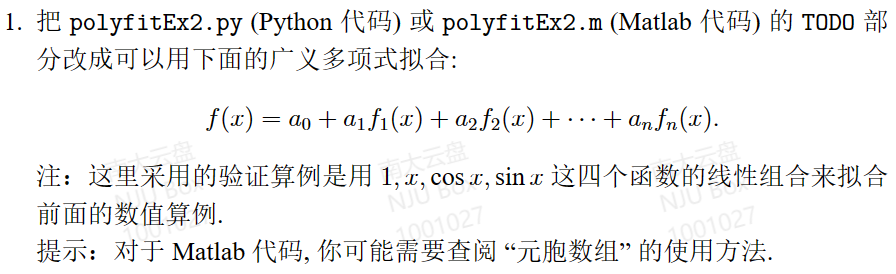
\includegraphics[width=\linewidth]{pics/7pro1.png}
        \end{figure}
    \subsection{算法思路}
    按照广义多项式拟合的方法补全代码:
    \lstset{
    numbers=left,
    language=Python,
    keywordstyle=\color{blue!100},
    commentstyle=\color{green!50!blue!50!},
    frame=shadowbox,%阴影
    escapeinside='',%英文分号输入中文
    xleftmargin=2em,xrightmargin=2em,aboveskip=1em,
    framexleftmargin=2em,
    extendedchars=false}

    \begin{lstlisting}[aboveskip=0pt]
        # TODO   
        xdatas[i] = f[i-1] (xdata)
    \end{lstlisting}
    之后使用 polyval 函数获取拟合的广义多项式函数的值,绘制出函数图像. 考虑使用函数族$f=(1,x,\cos x,\sin x)$进行拟合.
    \begin{algorithm}[H]
        \caption{由系数向量得到拟合函数值}
        \begin{algorithmic} %每行显示行号
            \Require 系数向量$a=(a_n,a_{n-1},\cdots,a_1,a_0)$,自变量向量$x$,\\拟合(广义)多项式族$f=(f_0,f_1,\cdots,f_{n-1},f_{n})$.
            \Ensure 函数值向量$y$
            \Function {polyval}{$a$, $x$, $f$}
                \State 翻转系数向量$a$
                \State $y_k \e a_0, \forall i$
                \For {$i$ 从 1 到 $n$}
                    \State $y \e a_i\cdot f_i(x)$
                \EndFor
                \State \Return $y$ 
            \EndFunction
        \end{algorithmic}
    \end{algorithm}
        \subsection{结果分析}
        与二次多项式拟合进行对比.
        \begin{figure}[H]
                \begin{minipage}{0.5\textwidth}
                    \centering
                    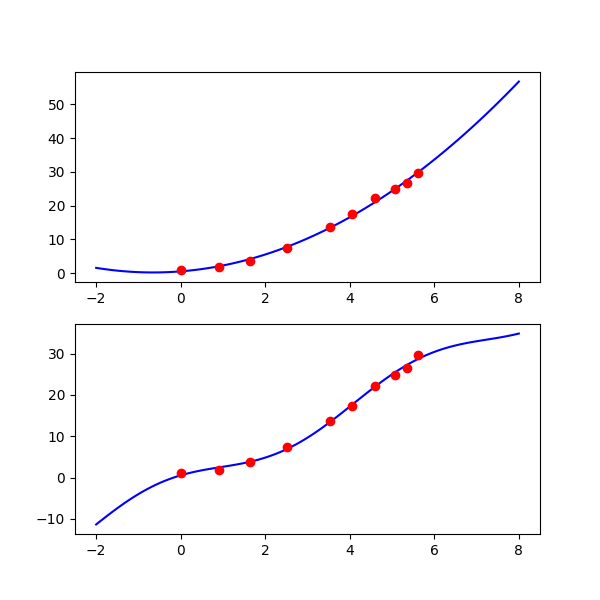
\includegraphics[width=\linewidth]{pics/P7.1.png}
                \end{minipage}%
                \begin{minipage}{0.5\textwidth}
                    \centering
                    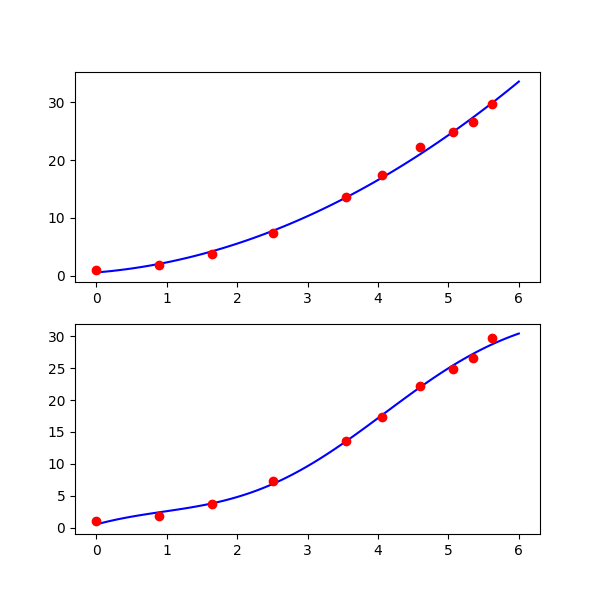
\includegraphics[width=\linewidth]{pics/P7.2.png}
                \end{minipage}
            \caption{二次多项式插值(上)与广义多项式插值(下)}
            \end{figure}
        可见多项式拟合与广义多项式在该批数据点上都有较好的拟合,将函数的定义域延展,可以观察到不同的效果,可以根据具体需求和更多的实际细节来选择拟合方式. 
\section{问题二} 
    \begin{figure}[H]
        \centering
        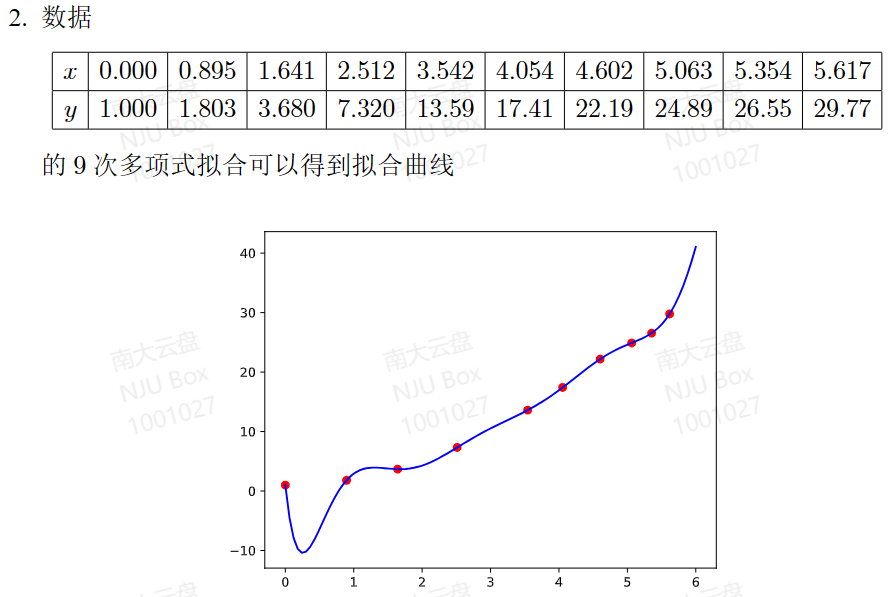
\includegraphics[width=\linewidth]{pics/7pro2.1.png}
        \end{figure}
    \begin{figure}[H]
        \centering
        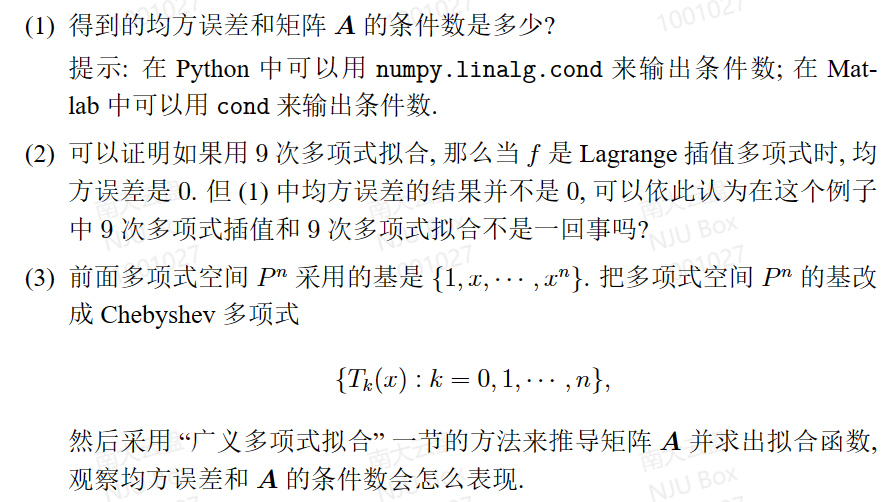
\includegraphics[width=\linewidth]{pics/7pro2.2.png}
        \end{figure}
    \subsection{算法思路}
    矩阵$A$的条件数是描述矩阵在数值计算中的稳定性和精度的指标. 它告诉我们矩阵在数值计算中对误差的敏感程度,具体来说,条件数越大,矩阵在计算过程中对误差越敏感. \par 均方误差的计算公式为$$\text{MSE}=\frac{1}{m}\sum_{i=1}^m(y_i-\hat{y}_i)^2$$\indent 根据9次多项式插值与9次多项式拟合的计算方法,可以得到它们的理论结果是完全一致的. 但是由于程序运行9次多项式拟合的过程中会出现数值计算的舍入误差及其累积,这会导致最终结果与理论结果有出入,所以命题(2)并不成立.\par Chebyshev 多项式可以通过递推关系得到:$$\left\{\begin{array}{l}
        T_0=1 \\
        T_1=x \\
        T_n=2xT_{n-1}-T_{n-2}, n\geqslant 2
        \end{array}\right.$$
    通过问题一中使用的广义多项式插值方法,同样可以得到使用 Chebyshev 多项式作为基底进行拟合的结果:$$f(x)=a_0T_0(x)+a_1T_1(x)+\cdots+a_nT_n(x)$$
    \subsection{结果分析}
        使用$\{1,x,x^2,\cdots,x^9\}$作为基底进行9次多项式拟合时,可以得到矩阵$A$的条件数与拟合函数的离散均方误差如下:$$\left\{\begin{array}{l}
            A_{\text{cond}}=8.578682559932301e+20 \\
            \text{MSE}=0.0004939324785567218
            \end{array}\right.$$
        这说明此时的矩阵$A$具有一定的病态性,但由于选点较少且并不极端,得到的拟合函数结果几乎没有离散误差,有着良好的拟合效果. \par 使用 Chebyshev 多项式 $\{1,x,T_2(x),\cdots,T_9(x)\}$作为基底进行9次多项式拟合时,可以得到矩阵$A$的条件数与拟合函数的离散均方误差如下:$$\left\{\begin{array}{l}
            A_{\text{cond}}=5.5388093317210355e+25 \\
            \text{MSE}=0.00017881211322257203
            \end{array}\right.$$
        $A$的条件数进一步增大但均方误差进一步减小,这应当与 Chebyshev 多项式的性质有关. 
        \begin{figure}[H]
            \begin{minipage}{0.5\textwidth}
                \centering
                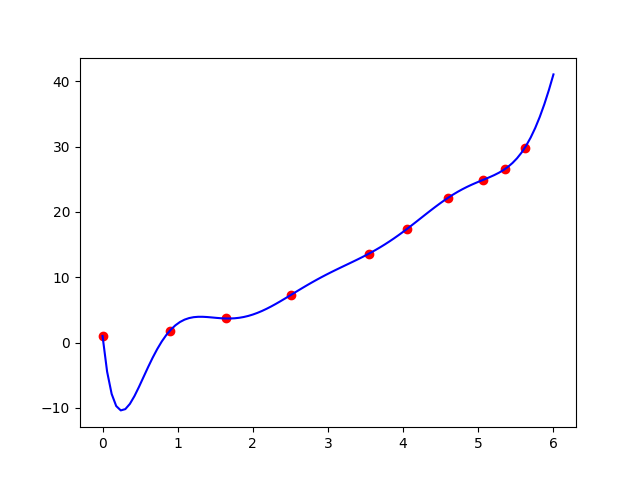
\includegraphics[width=\linewidth]{pics/P7.3.png}
            \end{minipage}%
            \begin{minipage}{0.5\textwidth}
                \centering
                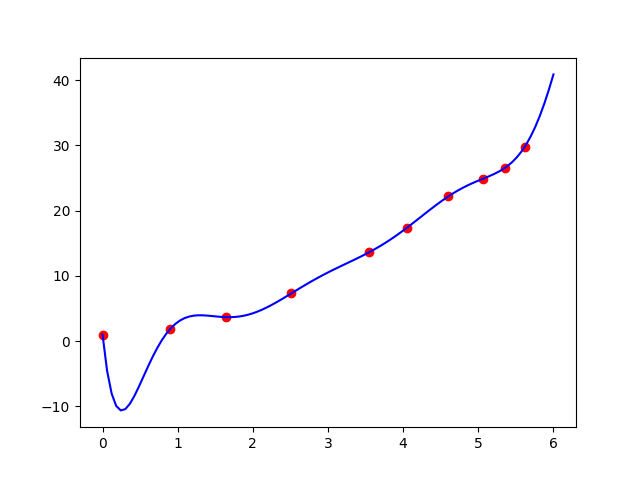
\includegraphics[width=\linewidth]{pics/P7.4.png}
            \end{minipage}
        \caption{9次多项式插值(左)与9次 Chebyshev 多项式插值(右)}
        \end{figure}
        
\section{问题三}
    \begin{figure}[H]
        \centering
        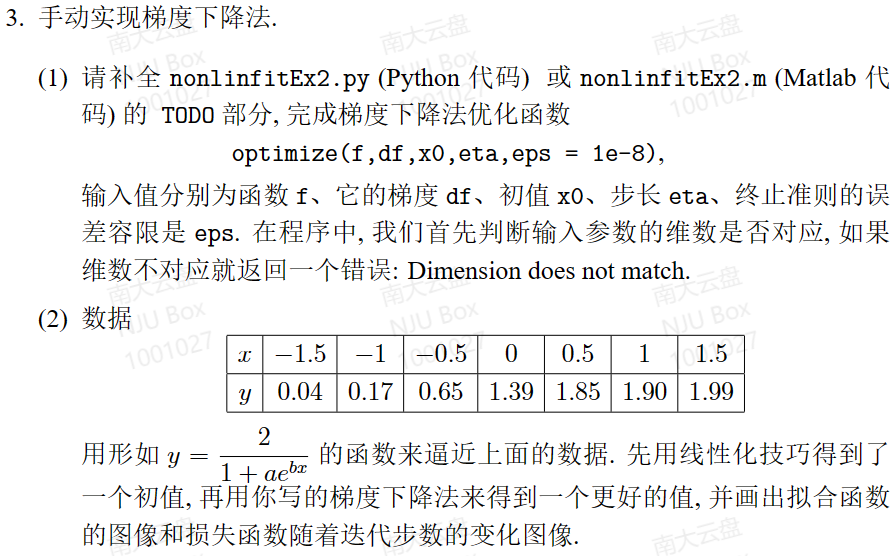
\includegraphics[width=\linewidth]{pics/7pro3.png}
        \end{figure}
    \subsection{算法分析}
    首先作一定的变换实现线性化:$$y=\frac{2}{1+a e^{b x}} \Leftrightarrow \frac{2}{y}=1+a e^{b x} \Leftrightarrow \ln \left(\frac{2}{y}-1\right)=bx+\ln a$$因此,取$u(x)=x$, $v(y)=\ln (\frac{2}{y}-1)$即可实现线性化. \par 课堂上介绍的梯度下降法的具体方法如下:
    \begin{algorithm}[H]
        \caption{梯度下降法}
        \begin{algorithmic} %每行显示行号
            \Require 多变量单值函数$f$, 梯度向量$\nabla f=(\frac{\partial f}{\partial x_1},\cdots,\frac{\partial f}{\partial x_n})$, 初始点$x_0=(x_0^1,\cdots,x_0^n)$, 学习率$\eta$, 最大收敛误差$eps$.
            \Ensure 最优值点$x_*=(x_*^1,\cdots,x_*^n)$
            \Function {optimize}{$f$, $\nabla f$, $x_0$, $\eta$, $eps$}
                \State $x_*=x_0$
                \For {$\left\lVert{\nabla f(x_*)} \right\rVert _2^2 > eps$}
                    \State $x_* \e x_* - \eta \nabla f(x_*)$
                \EndFor 
                \State \Return $x_*$ 
            \EndFunction
        \end{algorithmic}
    \end{algorithm}
    根据上述过程补全代码:
    \lstset{
    numbers=left,
    language=Python,
    keywordstyle=\color{blue!100},
    commentstyle=\color{green!50!blue!50!},
    frame=shadowbox,%阴影
    escapeinside='',%英文分号输入中文
    xleftmargin=2em,xrightmargin=2em,aboveskip=1em,
    framexleftmargin=2em,
    extendedchars=false}

    \begin{lstlisting}[aboveskip=0pt]
        # TODO   
        while True:
            gradient = np.array([dfi(*x) for dfi in df])
            x -= eta * gradient
            if np.linalg.norm(gradient) < eps:
                break
    \end{lstlisting}
    \par 本题中,梯度下降法选取的单值函数$f$为$loss$函数:$$\mathcal{L}(a, b)=\frac{1}{m} \sum_{i=1}^{m}\left|\frac{2}{1+a e^{b x_{i}}}-y_{i}\right|^{2}$$可以求得梯度向量$\nabla f=(\frac{\partial \mathcal{L}}{\partial a},\frac{\partial \mathcal{L}}{\partial b})$如下:$$\left\{\begin{array}{l}
        \frac{\partial \mathcal{L}}{\partial a} = \frac{1}{m} \sum_{i=1}^{m} \frac{-8e^{b x_{i}}}{\left(1+a e^{b x_{i}}\right)^2}  \cdot \left(\frac{2}{1+a e^{b x_{i}}} - y_{i}\right) \\
        \frac{\partial \mathcal{L}}{\partial b} = \frac{1}{m} \sum_{i=1}^{m} \frac{-8ax_i\cdot e^{b x_{i}}}{\left(1+a e^{b x_{i}}\right)^2} \cdot \left(\frac{2}{1+a e^{b x_{i}}} - y_{i}\right)
        \end{array}\right.$$
    固定$\eta=10^{-4}$, $eps=10^{-8}$进行优化. 
    \subsection{结果分析}
        \begin{figure}[H]
            \begin{minipage}{0.5\textwidth}
                \centering
                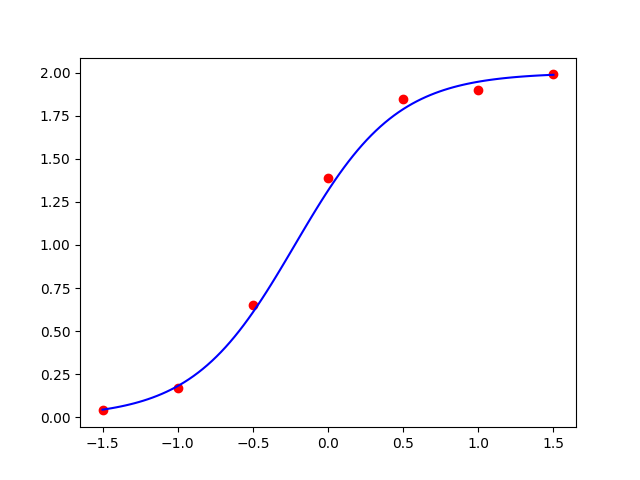
\includegraphics[width=\linewidth]{pics/P7.5.png}
            \end{minipage}%
            \begin{minipage}{0.5\textwidth}
                \centering
                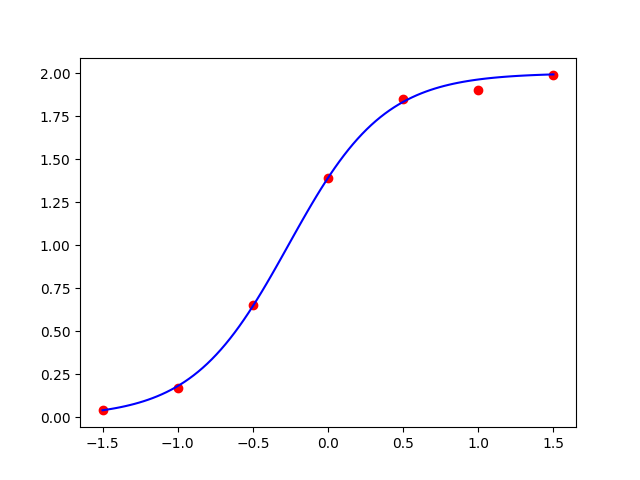
\includegraphics[width=\linewidth]{pics/P7.6.png}
            \end{minipage}
        \caption{梯度下降前(左)后(右)拟合函数图像}
        \end{figure}
        使用梯度下降法前的系数为$\left\{\begin{array}{l}
            a=0.5202092596711911 \\
            b=-2.9599994340662583
            \end{array}\right.$.使用梯度下降法后的系数为\\$\left\{\begin{array}{l}
                a=0.43798576249523435 \\
                b=-3.1320556568173634
                \end{array}\right.$再观察图像,可以看出梯度下降法有利于得到更好的局部最优解,得到效果更好的拟合函数. 梯度下降法的收敛函数(下图)也印证了这一点:
            \begin{figure}[H]
                \centering
                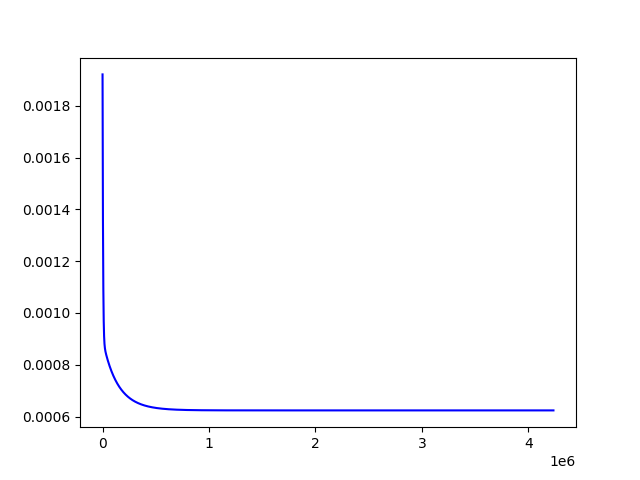
\includegraphics[width=0.6\linewidth]{pics/P7.7.png}
                \caption{梯度下降法$loss$值随迭代次数的变化}
            \end{figure}
            

\section{问题四}
    \begin{figure}[H]
        \centering
        
\includegraphics[width=\linewidth]{pics/7pro4.1.png}
        \end{figure}
    \begin{figure}[H]
        \centering
        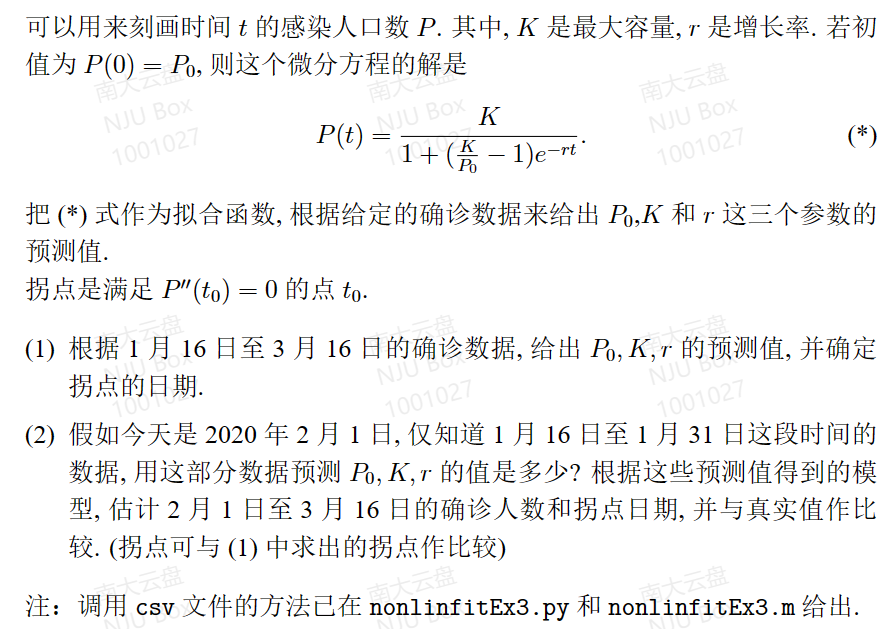
\includegraphics[width=\linewidth]{pics/7pro4.2.png}
        \end{figure}
    \subsection{算法分析}
    首先作一定的变换实现线性化:$$P(t)=\frac{K}{1+\left(\frac{K}{P_{0}}-1\right) e^{-r t}} \Leftrightarrow \ln [\frac{K}{P(t)}-1]=\ln (\frac{K}{P_0}-1)-rt$$因此,取$u(t)=-t$, $v(P)=\ln (\frac{K}{P}-1)$即可实现线性化$v=bu+c$, 并通过逆变换得到:$$\left\{\begin{array}{l}
        \frac{K}{P_0}=e^c+1 \\
        r=-b \\
        P_0=45 \quad \text{(观察数据可得)}
        \end{array}\right.$$
    便可以解出$P_0,K,r$的值. 为求出拐点$t_0$值,考虑对$P(t)$作二阶差分代替$P^{''}(t)$,即:$$P^{''}(t)\approx \frac{\Delta^2 P(t)}{{(\Delta t)}^2}=\frac{\frac{\Delta P(t+1)}{\Delta t}-\frac{\Delta P(t)}{\Delta t}}{\Delta t}=P(t+2)+P(t)-2\cdot P(t+1)$$则可以求出$t=t_0$为$P^{''}(t)$的零点. \par 使用同样的方法,也可以解决第二问的问题.
    \subsection{结果分析}
    \begin{figure}[H]
        \centering
        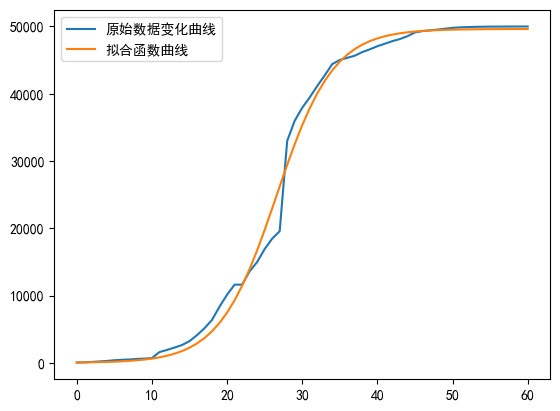
\includegraphics[width=0.6\linewidth]{pics/P7.8.png}
        \caption{Logistic 模型拟合函数图像}
    \end{figure}
    得到的参数值如下:$$\left\{\begin{array}{l}
        K=4.96346018e+04 \\
        r=2.63615937e-01 \\
        P_0=45
        \end{array}\right.$$
    \begin{figure}[H]
        \centering
        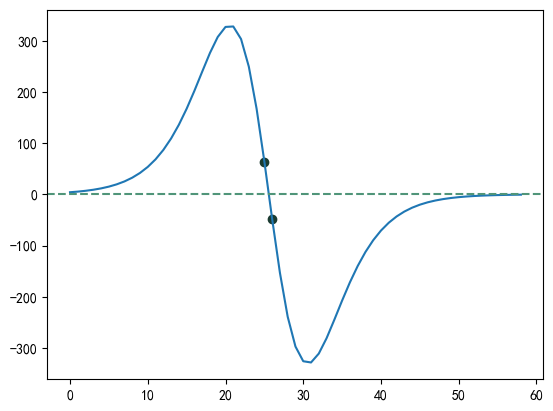
\includegraphics[width=0.6\linewidth]{pics/P7.9.png}
        \caption{拟合函数二阶差分图像}
    \end{figure}
    由图像可以得出,拐点的日期在2020/2/10与2020/2/11之间,即1月16日之后的25天到26天之间. \par 若只考虑1月16日至1月31日的数据,则有如下的拟合结果:
    \begin{figure}[H]
        \centering
        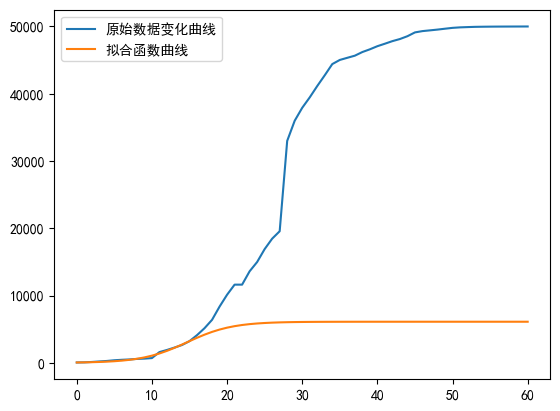
\includegraphics[width=0.6\linewidth]{pics/P7.10.png}
        \caption{Logistic 模型拟合函数图像}
    \end{figure}
    得到的参数值如下:$$\left\{\begin{array}{l}
        K=6.10376831e+03 \\
        r=3.34055875e-01 \\
        P_0=45
        \end{array}\right.$$
    \begin{figure}[H]
        \centering
        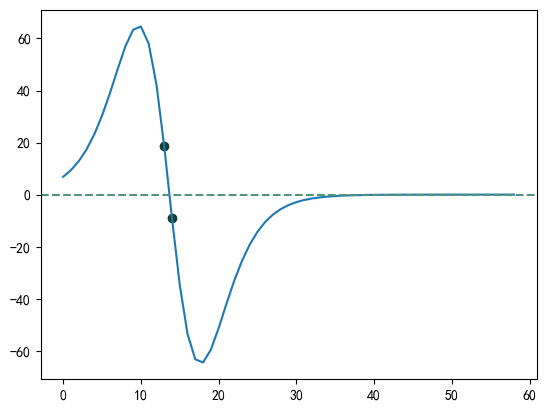
\includegraphics[width=0.6\linewidth]{pics/P7.11.png}
        \caption{拟合函数二阶差分图像}
    \end{figure}
    由图像可以得出,拐点的日期在2020/1/29与2020/1/30之间,即1月16日之后的13天到14天之间. 但可以看出,只使用前16天的数据,模型拟合的效果很不理想,说明实际的疫情演变需要考虑更多复杂的因素.
\section{结论}
    函数拟合分为线性拟合与非线性拟合,线性拟合的方法可以推广到多项式拟合与广义多项式拟合,非线性拟合可以通过一定的线性化手段实现将非线性拟合问题转化为一个线性拟合问题. 找到一个合适的参数向量后,可以通过梯度下降法进一步优化参数向量,得到更好的拟合效果.
\clearpage

\section{附录: 问题四完整程序代码}
\lstset{
    numbers=left,
    language=Python,
    keywordstyle=\color{blue!100},
    commentstyle=\color{green!50!blue!50!},
    frame=shadowbox,%阴影
    escapeinside='',%英文分号输入中文
    xleftmargin=2em,xrightmargin=2em,aboveskip=1em,
    framexleftmargin=2em,
    extendedchars=false}

\begin{lstlisting}[aboveskip=0pt]
import pandas as pd  #需要安装pandas包读取csv文件
# 读取数据
df = pd.read_csv('wuhan2020.csv')
df
df_save = df[df.index<61]
df_save
import numpy as np
t=np.array(df_save.index)
P=np.array(df_save['武汉市'])
print(t)
print(P)
from scipy.optimize import curve_fit
# 定义拟合函数
def func(t, K, r):
    return K / (1 + (K/45 - 1) * np.exp(-1 * r * t))
# 使用curve_fit进行拟合
popt, pcov = curve_fit(func, t, P, maxfev=100000)
# 输出拟合得到的参数值
print("拟合参数:", popt)
import matplotlib.pyplot as plt
plt.rcParams['font.sans-serif'] = ['SimHei']  # 指定默认字体
plt.rcParams['axes.unicode_minus'] = False  # 解决保存图像是负号'-'显示为方块的问题
plt.plot(t,P,label='原始数据变化曲线')
plt.plot(t,func(t,popt[0],popt[1]),label='拟合函数曲线')
plt.legend()
plt.show()
diff2=[]
for i in range(59):
    diff2.append(func(i+2,popt[0],popt[1])+func(i,popt[0],popt[1])-2*func(i+1,popt[0],popt[1]))
print(diff2)
plt.plot(t[:59],diff2)
plt.axhline(y=0, linestyle='--', color='#509579')
plt.scatter(25, diff2[25], color='#1a3b30')
plt.scatter(26, diff2[26], color='#1a3b30')
plt.show()
for i in range(59):
    if diff2[i]*diff2[i+1]<0:
        print('t0 =',i)
        break
df_save[df_save.index==25]
df_save[df_save.index==26]
df_save[df_save['日期']=='2020/2/1']
df_predict=df_save[df_save.index<16]
df_predict
t_pre=np.array(df_predict.index)
P_pre=np.array(df_predict['武汉市'])
popt, pcov = curve_fit(func, t_pre, P_pre, maxfev=100000)
print(popt)
plt.plot(t,P,label='原始数据变化曲线')
plt.plot(t,func(t,popt[0],popt[1]),label='拟合函数曲线')
plt.legend()
plt.show()
diff_2=[]
for i in range(59):
    diff_2.append(func(i+2,popt[0],popt[1])+func(i,popt[0],popt[1])-2*func(i+1,popt[0],popt[1]))
plt.plot(t[:59],diff_2)
plt.axhline(y=0, linestyle='--', color='#509579')
plt.scatter(13, diff_2[13], color='#1a3b30')
plt.scatter(14, diff_2[14], color='#1a3b30')
plt.show()
for i in range(59):
    if diff_2[i]*diff_2[i+1]<0:
        print('t0 =',i)
        break
df_save[df_save.index==13]
df_save[df_save.index==14]
\end{lstlisting}

\clearpage



\bibliographystyle{unsrt}
\bibliography{Reference}
\end{document}